\documentclass[11pt]{article}
\usepackage{amsmath}
\usepackage{graphicx}
\usepackage{amsthm}
\title{Background Info}


\setlength\parindent{0pt}
\author{Aneesh Malhotra Rishi Gupta, Adrienne Stotle,  Shakib Rashid}

\begin{document}
\maketitle
Our goal is to implement the 2-Dimensional Richardson Algorithm, which we will show an explanation of here

Given a degraded image, $H$, of size $N \times M$, and a (normalized) blurring kernel $S$, which is of size $K \times K$, we will need to recover the original image $W$, which must be of size $(N-K+1) \times (M - K +1)$. 

We will say $H,W,S$ are probability frequency functions, where the events describe energy at cells of the image, and that $P(W_{ij}) = \frac{W_{ij}}{\sum W}$

By Bayes' Theorem
\begin{align*}
P(W_{ij} | H_{nm}) &= \frac{P(H_{nm}|W_{ij})}{\sum \limits_{k,l}P(H_{nm} |W_{kl}) \cdot P(W_{kl})}
\end{align*}

Also

$$
P(W_i) = \sum \limits_{n,m} P(W_{ij}|H_{nm})\cdot P(H_{nm})
$$

Substituting in for $P(W_{ij} | H_{nm})$, we see that 

$$
P(W_{ij}) = \sum \limits_{n=0}^{N-1} \sum \limits_{m=0}^{M-1} \frac{P(H_{nm} | W_{ij}) P(H_{nm}) P(W_{ij})}{ \sum \limits_{\ell = 0}^{I-1} \sum \limits_{k=0}^{J-1} P(H_{nm}|W_{\ell k}) \cdot P(W_{\ell k})}
$$
To find the conditional probability $P(H_{nm}|W_{ij})$, consider an event at $W_{ij}$. We will denote this by a two-dimensional impulse, so $W_{ij} = \delta(i,j)$ Then by the sifting property,
\begin{align*}
H_{nm} &= \sum \limits_{p,q} S_{n-p,m-q} \delta(i,j) \\
H_{nm} &= S_{n-i,m-j}
\end{align*}
Therefore, 
\begin{align*}
P(H_{nm}|W_{ij}) &= \frac{S_{n-i,m-j}}{\sum \limits_{n,m} S_{n-i,m-j}} = P(S_{n-i,m-j})  \\
\end{align*}

\begin{align*}
P(W_{ij}) &= P(W_{ij}) \sum \limits_{n=0}^{N-1} \sum \limits_{m=0}^{M-1} \frac{P(S_{n-i,m-j}) P(H_{nm}) }{ \sum \limits_{\ell = 0}^{I-1} \sum \limits_{k=0}^{J-1} P(S_{n-\ell,m-k}) \cdot P(W_{\ell k})}
\end{align*}
Since convolution preserves total sum, we can cancel out the probabilities, and we will turn this into an iteration, where $r$ is the iteration number.

\begin{align*}
W_{ij,r+1} &= W_{ij,r} \sum \limits_{n=0}^{N-1} \sum \limits_{m=0}^{M-1} \frac{S_{n-i,m-j} H_{nm} }{ \sum \limits_{\ell = 0}^{I-1} \sum \limits_{k=0}^{J-1} S_{n-\ell,m-k}  W_{\ell k,r}}
\end{align*}
Since we we only need to consider positive indices of $S$, we can make this iteration by adjusting the summation indices.

\begin{align*}
W_{ij,r+1} &= W_{ij,r} \sum \limits_{n=i}^{N-1} \sum \limits_{m=j}^{M-1} \frac{S_{n-i,m-j} H_{nm} }{ \sum \limits_{\ell = 0}^{I-1} \sum \limits_{k=0}^{J-1} S_{n-\ell,m-k}  W_{\ell k,r}}
\end{align*}

We notice that these are convolutions, so 

$$W_{r+1} = W_{r}\cdot \left (S^{T} * \frac{H}{S*W_r} \right ).$$
This is the iteration we will compute.

Additionally, we will need to explore the effects of different point spread functions on our image. So far we have explored Gaussian blur kernels. 

The continuous point spread function with standard deviation
$$
f(x,y) = \frac{1}{2 \pi \sigma^2} \exp \left (   -\frac{1}{2}(x - \mu)^2 - \frac{1}{2}(y - \mu)^2) \right )
$$
When discretizing this distribution, we choose the interval to span 2 standard deviations in each direction. Additionally, we must choose how many pixels this kernel will integrate over, which will be determined by the size of the discretization


\begin{figure}
\centering
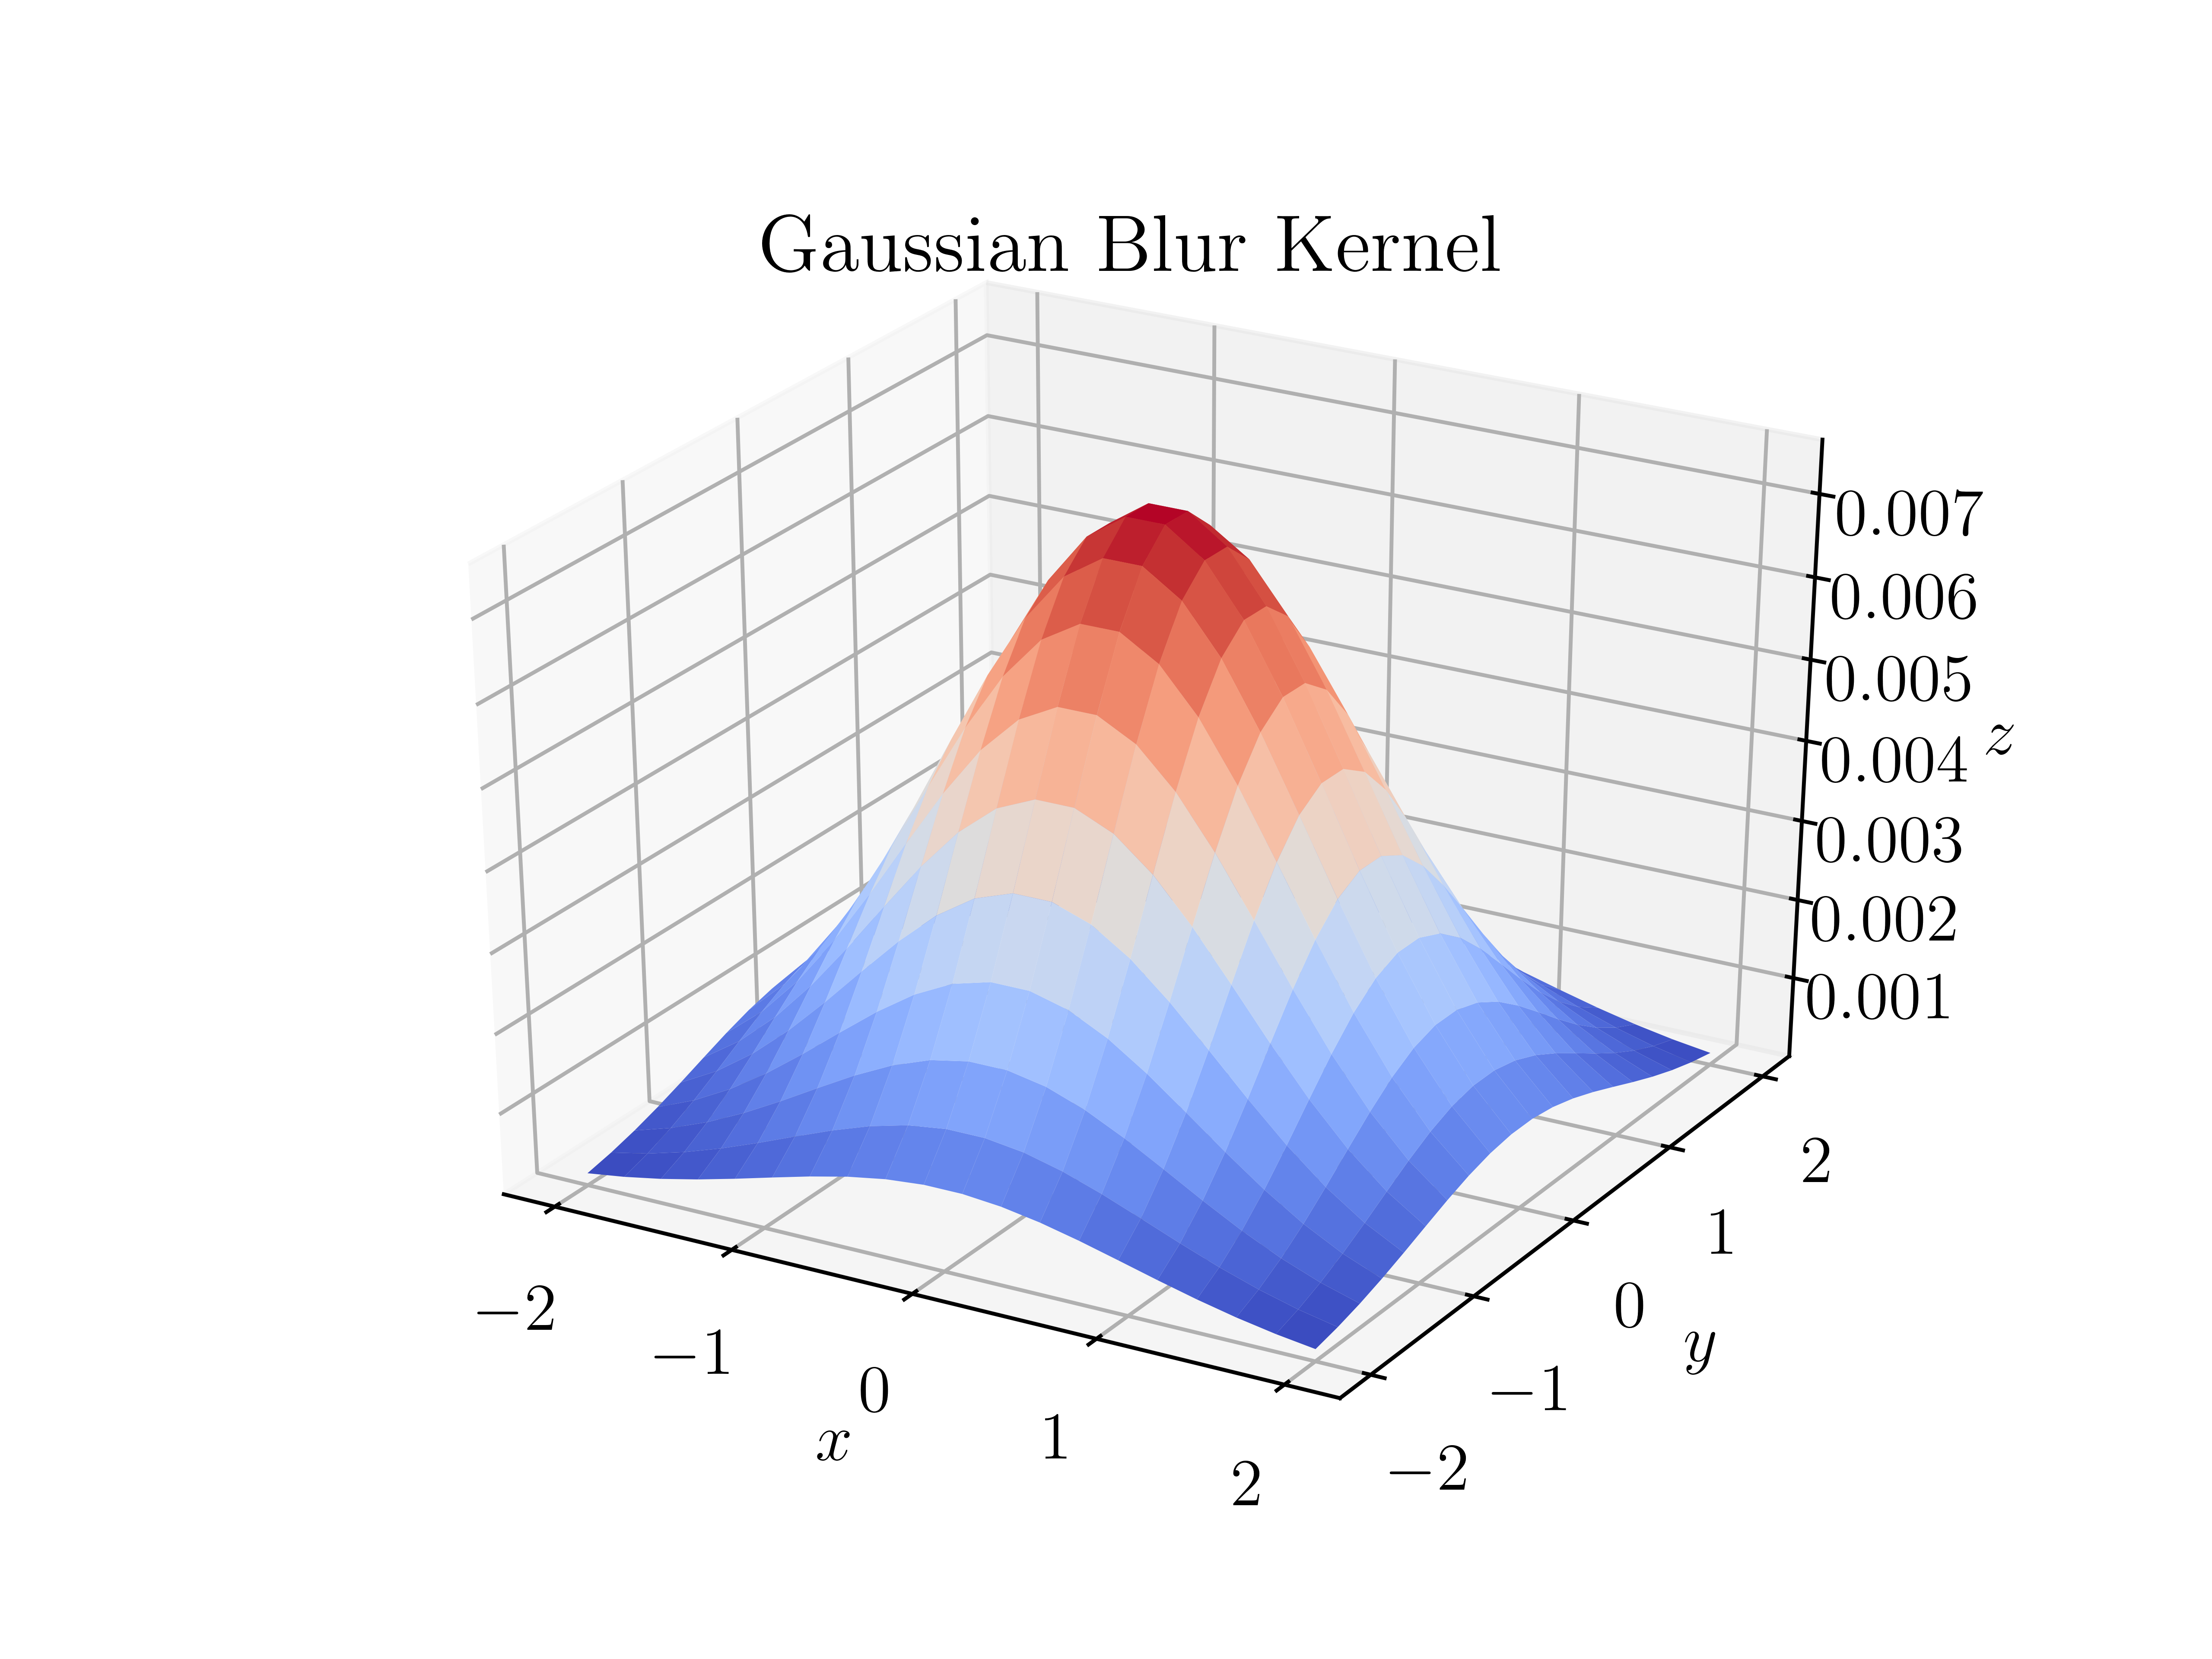
\includegraphics[scale = 0.8]{Gaussian.png}
\caption{ $20 \times 20$ Gaussian Blur with $\mu = 0$. and $\sigma^2 = 1$}
\end{figure}

\end{document}